% =============================================================================
% APRESENTAÇÃO COMPLETA DO PROJETO AM 2026.2 - SPAMBASE
% Base: projetoAM20262Q1-main (relatório final consolidado e resultados CSV)
% Formato inspirado no slides(1).tex: Beamer Madrid, 16:9, cores CIn/UFPE.
% Duracao planejada: 7min30 a 8min30 de exposicao + tempo de discussao.
% Os graficos sao referenciados diretamente em ../../../questao1 e ../../../questao2.
% Compilar: pdflatex -interaction=nonstopmode apresentacao_spambase_completa.tex (2x)
%
% Sugestao de participacao:
% Douglas: Q1 metodo; Felipe: Q1 resultados / Q2 protocolo; Leticia: Q2 resultados / estatistica. Ajustar para que todos participem.
% =============================================================================
\documentclass[aspectratio=169,11pt]{beamer}
\usetheme{Madrid}
\usepackage[utf8]{inputenc}
\usepackage[T1]{fontenc}
\usepackage{lmodern}
\usepackage[brazilian]{babel}
\usepackage{graphicx}
\usepackage{booktabs}
\usepackage{amsmath}
\usepackage{array}
\usepackage{tikz}
\usetikzlibrary{arrows.meta,positioning,calc}
\usepackage{pgfplots}
\pgfplotsset{compat=1.18}
\usepackage[most]{tcolorbox}

\definecolor{cinazul}{RGB}{0,51,102}
\definecolor{azulclaro}{RGB}{204,224,245}
\definecolor{cinzaescuro}{RGB}{90,90,90}
\definecolor{laranja}{RGB}{204,102,0}
\definecolor{verdeescuro}{RGB}{0,102,51}
\definecolor{ciano}{RGB}{26,129,153}
\definecolor{neutro}{RGB}{245,248,252}
\definecolor{bordacinza}{RGB}{218,226,235}

\setbeamercolor{structure}{fg=cinazul}
\setbeamercolor{frametitle}{bg=cinazul,fg=white}
\setbeamercolor{title}{fg=white,bg=cinazul}
\setbeamercolor{block title}{bg=cinazul,fg=white}
\setbeamercolor{block body}{bg=neutro,fg=black}
\setbeamercolor{alerted text}{fg=laranja}
\setbeamerfont{frametitle}{size=\large,series=\bfseries}
\setbeamertemplate{navigation symbols}{}
\setbeamersize{text margin left=0.72cm,text margin right=0.72cm}
\setbeamertemplate{footline}{%
  \leavevmode\hbox{%
    \begin{beamercolorbox}[wd=.78\paperwidth,ht=2.4ex,dp=1.0ex,leftskip=.65cm]{palette primary}%
      \tiny\color{white}IN1102 \hspace{1em} Spambase | Double K-means e Classificação
    \end{beamercolorbox}%
    \begin{beamercolorbox}[wd=.22\paperwidth,ht=2.4ex,dp=1.0ex,rightskip=.65cm plus1fil]{palette primary}%
      \hfill\tiny\color{white}CIn/UFPE \quad \insertframenumber/\inserttotalframenumber
    \end{beamercolorbox}%
  }%
}
\setbeamercolor{palette primary}{bg=cinazul,fg=white}
\setbeamertemplate{itemize items}[circle]
\setbeamertemplate{enumerate items}[default]

\newtcolorbox{notabox}[1][]{colback=azulclaro!38,colframe=cinazul!28,boxrule=.5pt,arc=2mm,
  left=2mm,right=2mm,top=1.4mm,bottom=1.4mm,#1}
\newtcolorbox{alertabox}[1][]{colback=laranja!7,colframe=laranja!65,boxrule=.7pt,arc=2mm,
  left=2.5mm,right=2.5mm,top=1.5mm,bottom=1.5mm,#1}
\newtcolorbox{simplebox}[1][]{colback=neutro,colframe=bordacinza,boxrule=.55pt,arc=2mm,
  left=2.2mm,right=2.2mm,top=2mm,bottom=2mm,#1}

\newcommand{\kpi}[3]{%
\begin{tcolorbox}[colback=#3!8,colframe=#3!32,boxrule=.55pt,arc=2mm,
  halign=center,left=1mm,right=1mm,top=1.8mm,bottom=1.8mm]
{\fontsize{23}{24}\selectfont\bfseries\color{#3}#1}\\[1mm]
{\footnotesize #2}
\end{tcolorbox}}

\newcommand{\scorebar}[4]{%
\begin{tikzpicture}[x=1cm,y=1cm,baseline=0]
\node[anchor=east,font=\scriptsize,text width=2.12cm,align=right] at (2.15,0) {#1};
\fill[cinazul!8] (2.33,-.145) rectangle (8.83,.145);
\fill[#4] (2.33,-.145) rectangle ({2.33+6.5*#2},.145);
\node[anchor=west,font=\small\bfseries,color=cinazul] at (8.99,0) {#3};
\end{tikzpicture}\par\vspace{2mm}}

\title[Spambase | Apresentação completa]{\textbf{Spambase: do co-clustering à classificação}}
\subtitle{Double K-means, cinco classificadores e comparação estatística}
\author[Douglas, Felipe e Leticia]{Douglas Ara\'ujo Silva \quad Felipe Ara\'ujo de Lima \\ Let\'icia De Albuquerque S. Leit\~ao}
\institute[CIn/UFPE]{Aprendizagem de M\'aquina -- IN1102 | P\'os-gradua\c c\~ao, CIn/UFPE}
\date{18 de novembro de 2026}

\begin{document}

\begin{frame}[plain]
\vspace{5mm}
\titlepage
\begin{center}\begin{tikzpicture}
\fill[cinazul] (0,0) rectangle (2.1,.06);
\fill[laranja] (2.2,0) rectangle (2.9,.06);
\fill[verdeescuro] (3.0,0) rectangle (5.1,.06);
\end{tikzpicture}\end{center}
\end{frame}

%% PRINCIPAL 2
\begin{frame}[t]{O projeto em duas questões}

\begin{columns}[T,onlytextwidth]
\column{.32\textwidth}\kpi{4.601}{e-mails}{cinazul}
\column{.32\textwidth}\kpi{57}{atributos numéricos}{ciano}
\column{.32\textwidth}\kpi{2 + 3}{classes dos dois alvos}{verdeescuro}
\end{columns}
\vspace{2mm}
\begin{columns}[T,onlytextwidth]
\column{.48\textwidth}\begin{simplebox}
\textbf{Q1: não supervisionada}\par\smallskip
\small Co-clustering de objetos e variáveis.\par
\small $K\in\{2,3,4\}$, $H\in\{1,\ldots,K\}$; selecionar $K^*$ pela Silhueta.
\end{simplebox}
\column{.48\textwidth}\begin{simplebox}
\textbf{Q2: supervisionada}\par\smallskip
\small Cinco classificadores em dois alvos: rótulo original (2 classes) e clusters encontrados em Q1 (3 classes).
\end{simplebox}\end{columns}
\vspace{2mm}\scriptsize Rótulo original: 2.788 não-spam (60,6\%) e 1.813 spam (39,4\%).

\end{frame}

%% PRINCIPAL 3
\begin{frame}[t]{Q1 | O que o Double K-means otimiza?}

\begin{columns}[T,onlytextwidth]
\column{.53\textwidth}
\begin{tikzpicture}[>=Stealth,node distance=5mm,
box/.style={draw=cinazul!35,fill=neutro,rounded corners=2pt,text width=4.85cm,inner sep=3pt,minimum height=.77cm,font=\small,align=center}]
\node[box] (x) {Dados $X$: objetos $\times$ atributos};
\node[box,below=of x] (uv) {$U$: grupos dos e-mails ($K$); $V$: grupos de atributos ($H$)};
\node[box,below=of uv] (g) {$G$: médias de cada um dos $K\times H$ blocos};
\node[box,below=of g] (a) {Atualizar $G$, $U$ e $V$ alternadamente};
\draw[->,thick,cinazul] (x)--(uv);\draw[->,thick,cinazul] (uv)--(g);\draw[->,thick,cinazul] (g)--(a);
\end{tikzpicture}
\column{.44\textwidth}
\begin{simplebox}
\small \textbf{Função objetivo}\par
\[\textstyle W=\sum_{k,h,i,j}u_{ik}v_{jh}(x_{ij}-g_{kh})^2\]
\small Minimiza a variabilidade dentro dos blocos.
\end{simplebox}
\vspace{1mm}
\begin{notabox}\small Parada por partições estáveis ou por $200$ iterações.\end{notabox}
\end{columns}

\end{frame}

%% PRINCIPAL 4
\begin{frame}[t]{Q1 | Protocolo: 9 pares e 100 reinícios}

\begin{columns}[T,onlytextwidth]
\column{.32\textwidth}\kpi{9}{pares $(K,H)$}{cinazul}
\column{.32\textwidth}\kpi{100}{rodadas válidas por par}{ciano}
\column{.32\textwidth}\kpi{900}{execuções por representação}{laranja}
\end{columns}
\vspace{3mm}
\begin{enumerate}
\setlength{\itemsep}{5pt}
\item Para cada $(K,H)$: manter a \textbf{solução de menor $W$} entre 100 reinícios válidos.
\item Para cada par vencedor: calcular a \textbf{Silhueta Euclidiana média}.
\item Selecionar $(K^*,H^*)=\arg\max_{K,H}\operatorname{Sil}(K,H)$.
\item Depois de fixar a partição: medir \textbf{ARI} frente aos rótulos originais.
\end{enumerate}
\begin{notabox}\scriptsize Grade: $(2,1),(2,2),(3,1),(3,2),(3,3),(4,1),(4,2),(4,3),(4,4)$. Grupos vazios invalidam uma tentativa.\end{notabox}

\end{frame}

%% PRINCIPAL 5
\begin{frame}[t]{Q1 | Silhueta alta nem sempre é boa partição}

\begin{columns}[T,onlytextwidth]
\column{.43\textwidth}
\begin{simplebox}\centering
\small \textbf{Linha de base: z-score puro}\par\vspace{2mm}
{\fontsize{23}{24}\selectfont\bfseries\color{laranja}0,6596}\\\scriptsize Silhueta média\\[2mm]
{\fontsize{23}{24}\selectfont\bfseries\color{cinazul}$-0,00495$}\\\scriptsize ARI\\[1mm]
\small $(K^*,H^*)=(2,2)$
\end{simplebox}
\column{.54\textwidth}
\begin{notabox}
\textbf{O que foi isolado?}\par\smallskip
\small Apenas \textbf{34 e-mails não-spam} (0,74\%), associados a 11 termos técnicos raros, versus 4.567 outros e-mails.
\end{notabox}
\vspace{2mm}
\begin{alertabox}\small \textbf{Interpretação:} Silhueta mede geometria da partição; ARI mede concordância com as classes externas.\end{alertabox}
\end{columns}

\end{frame}

%% PRINCIPAL 6
\begin{frame}[t]{Q1 | Decisão sobre o pré-processamento}

\small Foram avaliadas \textbf{sete representações} (6.300 execuções válidas ao todo).\vspace{2mm}
\par
\scriptsize
\renewcommand{\arraystretch}{1.03}
\setlength{\tabcolsep}{4pt}
\centering
\begin{tabular}{lccc}
\toprule
Representação & $(K^*,H^*)$ & Silhueta & ARI \\
\midrule
z-score (`revisada`) & $(2,2)$ & 0,6596 & -0,00495 \\
Binarização + z-score & $(3,3)$ & 0,2100 & 0,2695 \\
\textbf{log1p + MinMax} & \textbf{$(3,3)$} & \textbf{0,1292} & \textbf{0,3911} \\
Quantis uniformes & $(3,3)$ & 0,1903 & 0,2925 \\
Clip + log + z-score & $(2,1)$ & 0,1721 & 0,1292 \\
Filtragem de domínio & $(2,1)$ & 0,2926 & 0,1363 \\
Z-score parcial nas maiúsculas & $(2,2)$ & 0,6537 & -0,00495 \\
\bottomrule
\end{tabular}
\par
\vspace{2mm}
\begin{alertabox}\scriptsize \textbf{Transparência:} $(K,H)$ foi escolhido pela Silhueta \emph{em cada representação}; a decisão posterior de usar \texttt{log\_minmax} também considerou ARI conhecido. Não foi totalmente cega aos rótulos.\end{alertabox}

\end{frame}

%% PRINCIPAL 7
\begin{frame}[t]{Q1 | Silhueta $\times$ $(K,H)$ na solução adotada}

\begin{columns}[T,onlytextwidth]
\column{.73\textwidth}\centering 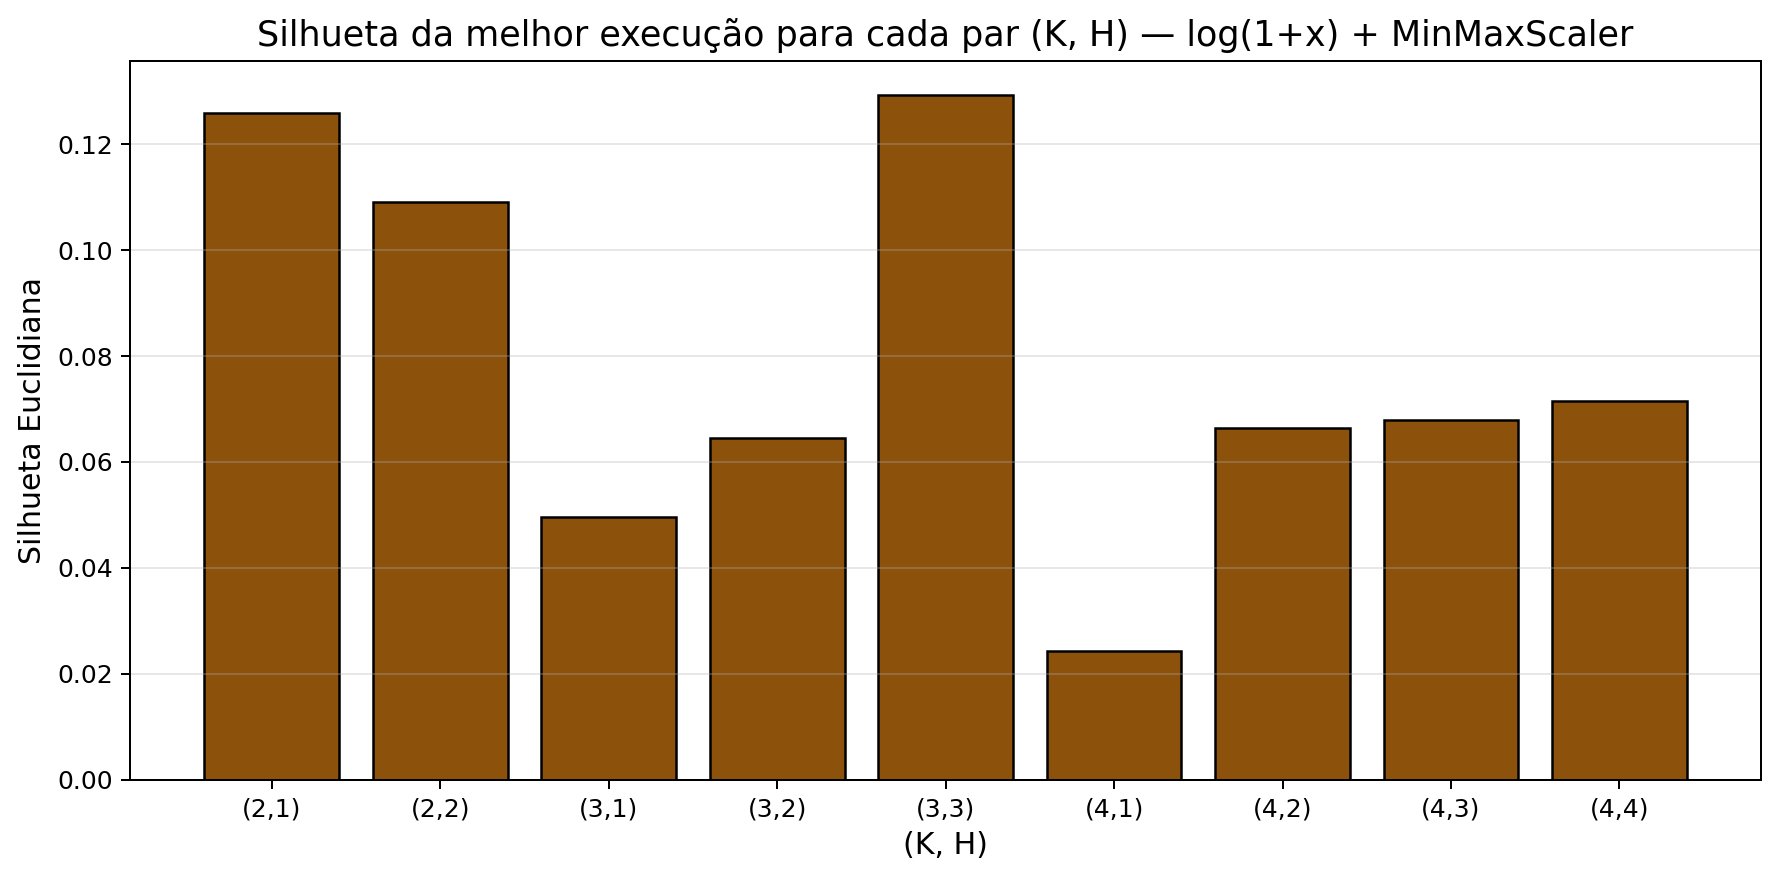
\includegraphics[width=\linewidth,height=5.6cm,keepaspectratio]{../../../questao1/resultados/log_minmax/silhouette_KH.png}
\column{.25\textwidth}
\begin{simplebox}\centering
{\Large\bfseries\color{verdeescuro}$(3,3)$}\\\scriptsize maior Silhueta entre os nove pares da representação \texttt{log\_minmax}\\[3mm]
{\large\bfseries 0,129219}\\\scriptsize Silhueta
\end{simplebox}
\vspace{2mm}\scriptsize \textbf{Regra correta:} primeiro menor $W$; depois maior Silhueta.
\end{columns}

\end{frame}

%% PRINCIPAL 8
\begin{frame}[t]{Q1 | Matriz de protótipos dos blocos $G$}

\small Médias da representação $\log(1+x)$ + MinMax, em $[0,1]$.\vspace{2mm}
\par
\small
\renewcommand{\arraystretch}{1.65}
\setlength{\tabcolsep}{4pt}
\centering
\begin{tabular}{lccc}
\toprule
Grupo de e-mails & $G_{\cdot,0}$ (4 var.) & $G_{\cdot,1}$ (31 var.) & $G_{\cdot,2}$ (22 var.) \\
\midrule
Cluster 0 (2.619) & 0,194479 & 0,022612 & 0,025559 \\
Cluster 1 (265) & 0,240859 & \textbf{0,132449} & 0,024273 \\
Cluster 2 (1.717) & \textbf{0,420265} & 0,008495 & \textbf{0,090361} \\
\bottomrule
\end{tabular}
\par
\vspace{3mm}
\begin{columns}[T,onlytextwidth]
\column{.32\textwidth}\begin{simplebox}\scriptsize \textbf{Grupo 0}\par Maiúsculas (longest/total), ``you'', ``your''.\end{simplebox}
\column{.32\textwidth}\begin{simplebox}\scriptsize \textbf{Grupo 1}\par Termos técnicos e frequências contextuais.\end{simplebox}
\column{.32\textwidth}\begin{simplebox}\scriptsize \textbf{Grupo 2}\par Termos comerciais, ``!'' e ``\$''.\end{simplebox}
\end{columns}

\end{frame}

%% PRINCIPAL 9
\begin{frame}[t]{Q1 | Matriz de contingência dos clusters}

\small Partição não supervisionada versus classes \emph{a priori} da base.\vspace{2mm}
\par
\small
\renewcommand{\arraystretch}{1.45}
\setlength{\tabcolsep}{4pt}
\centering
\begin{tabular}{lcccc}
\toprule
Cluster & Não-spam (0) & Spam (1) & Total & Predominância \\
\midrule
Cluster 0 & \textbf{2.218} & 401 & 2.619 & 84,69\% não-spam \\
Cluster 1 & \textbf{265} & 0 & 265 & 100\% não-spam \\
Cluster 2 & 305 & \textbf{1.412} & 1.717 & 82,24\% spam \\
Total & 2.788 & 1.813 & 4.601 &  \\
\bottomrule
\end{tabular}
\par
\vspace{3mm}
\begin{notabox}\small \textbf{ARI = 0,391111}: concordância externa parcial, superior à linha de base ($-0,00495$). O cluster 2 reúne $1.412$ de $1.813$ spams, mas não há correspondência perfeita entre clusters e classes.\end{notabox}

\end{frame}

%% PRINCIPAL 10
\begin{frame}[t]{Q1 | Evolução de $W$ e resultado final}

\begin{columns}[T,onlytextwidth]
\column{.69\textwidth}\centering 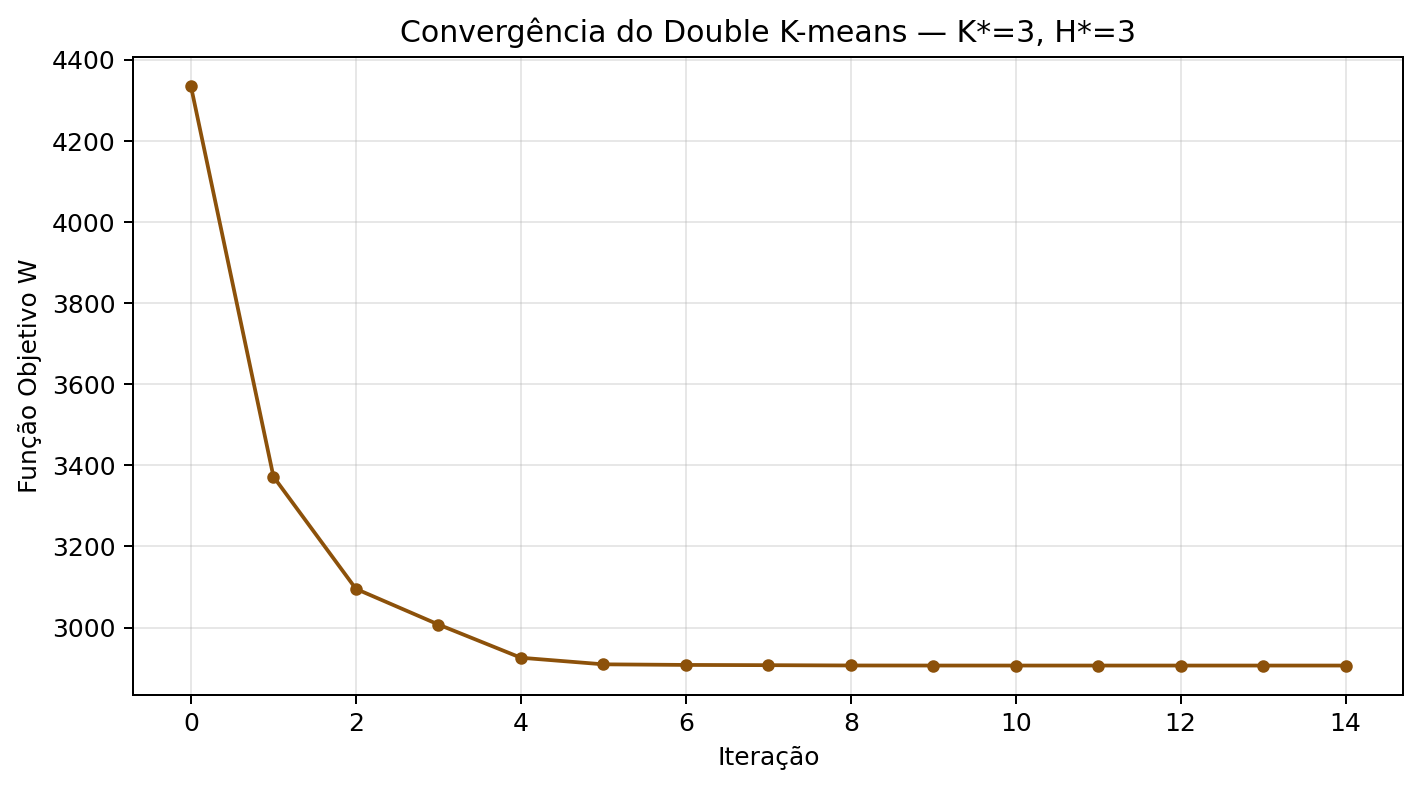
\includegraphics[width=\linewidth,height=5.55cm,keepaspectratio]{../../../questao1/resultados/log_minmax/objetivo_iteracoes.png}
\column{.29\textwidth}
\begin{simplebox}\centering
{\large\bfseries 14}\\\scriptsize iterações até convergir\\[3mm]
{\large\bfseries 2.906,23}\\\scriptsize $W$ final\\[3mm]
{\large\bfseries 33.044}\\\scriptsize melhor semente
\end{simplebox}
\vspace{2mm}\scriptsize A convergência corresponde à melhor execução válida de $(K,H)=(3,3)$.
\end{columns}

\end{frame}

%% PRINCIPAL 11
\begin{frame}[t]{Q1 $\rightarrow$ Q2 | Dois alvos, mesmos preditores}

\begin{columns}[T,onlytextwidth]
\column{.48\textwidth}\begin{simplebox}
\textbf{Versão A: rótulo original}\par\smallskip
\centering {\Large\bfseries 2 classes}\\\small 2.788 não-spam | 1.813 spam
\end{simplebox}
\column{.48\textwidth}\begin{simplebox}
\textbf{Versão B: cluster descoberto}\par\smallskip
\centering {\Large\bfseries 3 classes}\\\small 2.619 | 265 | 1.717 e-mails
\end{simplebox}
\end{columns}
\vspace{2mm}
\begin{notabox}\small Os \textbf{57 preditores} foram exportados em escala bruta. Em Q2, o \texttt{log1p + MinMax} é ajustado apenas no treino do fold (\textit{Pipeline}).\end{notabox}
\vspace{2mm}
\begin{alertabox}\scriptsize \textbf{Limitação transdutiva:} o agrupamento da Versão B foi aprendido sobre toda a base. A tarefa supervisionada mede a reprodução de rótulos fixos, não a generalização de clusters inéditos.\end{alertabox}

\end{frame}

%% PRINCIPAL 12
\begin{frame}[t]{Q2 | Cinco classificadores avaliados}

\begin{columns}[T,onlytextwidth]
\column{.48\textwidth}
\begin{simplebox}\small \textbf{1. Bayes Gaussiano multivariado}\par\scriptsize Prioris empíricas; média/covariância por classe; covariância ML \textbf{regularizada}.\end{simplebox}
\begin{simplebox}\small \textbf{2. Bayes k-vizinhos}\par\scriptsize Posteriori pela proporção entre $k$ vizinhos; três distâncias candidatas.\end{simplebox}
\begin{simplebox}\small \textbf{3. Bayes Parzen}\par\scriptsize Densidade por produto de kernels gaussianos; janela $h$.\end{simplebox}
\column{.48\textwidth}
\begin{simplebox}\small \textbf{4. Regressão Logística}\par\scriptsize Regularização $L_2$, ajuste de $C$ e peso das classes; softmax para 3 classes.\end{simplebox}
\begin{simplebox}\small \textbf{5. Voto Majoritário}\par\scriptsize Votos dos quatro modelos; desempate pela priori do treino externo.\end{simplebox}
\vspace{1mm}\begin{notabox}\scriptsize Pré-processamento idêntico por modelo: \texttt{log1p + MinMax} dentro de cada \textit{Pipeline}.\end{notabox}
\end{columns}

\end{frame}

%% PRINCIPAL 13
\begin{frame}[t]{Q2 | Validação cruzada aninhada e estratificada}

\begin{columns}[T,onlytextwidth]
\column{.5\textwidth}
\begin{tikzpicture}[>=Stealth,node distance=3.5mm,
box/.style={draw=cinazul!35,fill=azulclaro!25,rounded corners=2pt,text width=4.70cm,align=center,minimum height=.82cm,font=\small}]
\node[box] (a) {\textbf{30 repetições $\times$ 10 folds externos}\\9 treino | 1 teste};
\node[box,below=of a] (b) {\textbf{5-folds internos}\\Seleção de hiperparâmetros por F1 macro};
\node[box,below=of b] (c) {\textbf{Reajustar nos 9 folds}\quad e avaliar só no 10º};
\draw[->,thick,cinazul] (a)--(b);\draw[->,thick,cinazul] (b)--(c);
\end{tikzpicture}
\column{.46\textwidth}
\begin{simplebox}\centering
{\Large\bfseries 300}\\\scriptsize folds externos por modelo e alvo\\[2mm]
{\Large\bfseries 3.000}\\\scriptsize avaliações externas (5 modelos $\times$ 2 alvos)\\[2mm]
{\Large\bfseries 1.380.300}\\\scriptsize predições fora do treino
\end{simplebox}
\end{columns}
\vspace{2mm}\begin{notabox}\scriptsize Mesmos índices de folds para os cinco modelos; \texttt{Pipeline} evita vazamento de pré-processamento. Cada repetição testa todos os 4.601 e-mails exatamente uma vez.\end{notabox}

\end{frame}

%% PRINCIPAL 14
\begin{frame}[t]{Q2 | Hiperparâmetros pesquisados por 5-fold CV}

\par
\scriptsize
\renewcommand{\arraystretch}{1.32}
\setlength{\tabcolsep}{4pt}
\centering
\begin{tabular}{lp{2.15cm}p{6.35cm}c}
\toprule
Modelo & Parâmetro & Grade & Candidatos \\
\midrule
Gaussiano & Regularização $\lambda$ & {$10^{-6},10^{-4},10^{-2},10^{-1}$} & 4 \\
Bayes k-NN & $k$ e distância & $k=1,3,5,7,11,15,21$; Euclidiana, Manhattan, Chebyshev & 21 \\
Parzen & Largura $h$ & $0,04;0,08;0,12;0,20;0,35;0,55$ & 6 \\
Logística & $C$ e pesos & 5 valores de $C$: $0,03$ a $300$; peso padrão / balanceado & 10 \\
Voto & Sem tuning novo & Combina predições dos 4 modelos nos mesmos folds & -- \\
\bottomrule
\end{tabular}
\par
\vspace{2mm}
\begin{notabox}\scriptsize Critério de escolha interno: \textbf{maior F1 macro médio}; após a escolha, refaz-se o ajuste sobre os 9 folds externos de treinamento, sem usar o fold de teste.\end{notabox}

\end{frame}

%% PRINCIPAL 15
\begin{frame}[t]{Q2 | Como cada modelo foi avaliado?}

\begin{columns}[T,onlytextwidth]
\column{.49\textwidth}
\begin{simplebox}\small \textbf{Taxa de erro}\\[2mm]
\[\textstyle 1-\frac{n_{\mathrm{acertos}}}{n_{\mathrm{total}}}\]
\scriptsize Menor é melhor.
\end{simplebox}
\begin{simplebox}\small \textbf{Precisão macro}\\[1mm]
\[\textstyle \frac{1}{C}\sum_{c=1}^{C}\frac{TP_c}{TP_c+FP_c}\]
\scriptsize Menos falsos positivos por classe.
\end{simplebox}
\column{.49\textwidth}
\begin{simplebox}\small \textbf{Cobertura (recall) macro}\\[1mm]
\[\textstyle \frac{1}{C}\sum_{c=1}^{C}\frac{TP_c}{TP_c+FN_c}\]
\scriptsize Menos falsos negativos por classe.
\end{simplebox}
\begin{simplebox}\small \textbf{F1 macro}\\[1mm]
\[\textstyle \frac{1}{C}\sum_{c=1}^{C}\frac{2P_cR_c}{P_c+R_c}\]
\scriptsize Equilibra precisão e cobertura.
\end{simplebox}
\end{columns}
\vspace{1mm}\scriptsize Macro evita que a classe minoritária de 265 e-mails fique escondida pela média ponderada.

\end{frame}

%% PRINCIPAL 16
\begin{frame}[t]{Q2 | Resultados: classes originais (2 classes)}
\small Médias de 30 repetições de 10 folds; a tabela completa com ICs de 95\% está no apêndice.\vspace{2mm}
\par
\small
\renewcommand{\arraystretch}{1.3}
\setlength{\tabcolsep}{4pt}
\centering
\begin{tabular}{lcccc}
\toprule
Modelo & Erro $\downarrow$ & Precisão $\uparrow$ & Cobertura $\uparrow$ & F1 $\uparrow$ \\
\midrule
Gaussiano & 15,16\% & 0,8525 & 0,8683 & 0,8471 \\
Bayes k-NN & 6,74\% & 0,9321 & 0,9266 & 0,9290 \\
Bayes Parzen & 5,75\% & 0,9422 & 0,9372 & 0,9394 \\
Logística & 6,16\% & 0,9357 & 0,9359 & 0,9355 \\
Voto & 5,71\% & 0,9439 & 0,9364 & 0,9397 \\
\bottomrule
\end{tabular}
\par\vspace{3mm}
\begin{notabox}\small \textbf{Voto}: F1 $0,9397$ e erro $5,71\%$; \textbf{Parzen}: F1 $0,9394$ e erro $5,75\%$. Desempenhos muito próximos.\end{notabox}
\end{frame}

%% PRINCIPAL 17
\begin{frame}[t]{Q2 | Resultados: rótulos dos clusters (3 classes)}
\small Médias de 30 repetições de 10 folds; a tabela completa com ICs de 95\% está no apêndice.\vspace{2mm}
\par
\small
\renewcommand{\arraystretch}{1.3}
\setlength{\tabcolsep}{4pt}
\centering
\begin{tabular}{lcccc}
\toprule
Modelo & Erro $\downarrow$ & Precisão $\uparrow$ & Cobertura $\uparrow$ & F1 $\uparrow$ \\
\midrule
Gaussiano & 16,99\% & 0,7624 & 0,8774 & 0,7976 \\
Bayes k-NN & 6,55\% & 0,9392 & 0,8903 & 0,9114 \\
Bayes Parzen & 5,66\% & 0,9521 & 0,9000 & 0,9224 \\
Logística & 0,95\% & 0,9840 & 0,9819 & 0,9827 \\
Voto & 4,64\% & 0,9612 & 0,9141 & 0,9347 \\
\bottomrule
\end{tabular}
\par\vspace{3mm}
\begin{notabox}\small \textbf{Logística}: F1 $0,9827$ e erro $0,95\%$; reproduz especialmente bem a partição do Double K-means.\end{notabox}
\end{frame}

%% PRINCIPAL 18
\begin{frame}[t]{Q2 | Friedman: os cinco modelos diferem?}

\small $H_0$: desempenho equivalente em ranks médios; $n=30$ repetições pareadas, $k=5$ modelos.\vspace{2mm}
\par
\scriptsize
\renewcommand{\arraystretch}{1.1}
\setlength{\tabcolsep}{4pt}
\centering
\begin{tabular}{llccc}
\toprule
Alvo & Métrica & $\chi^2$ & $p$ (Friedman) & Rejeita $H_0$? \\
\midrule
Original & Erro & 114,52 & $7,91\times 10^{-24}$ & Sim \\
Original & Precisão & 115,89 & $4,02\times 10^{-24}$ & Sim \\
Original & Cobertura & 98,24 & $2,33\times 10^{-20}$ & Sim \\
Original & F1 macro & 114,24 & $9,07\times 10^{-24}$ & Sim \\
Clusters & Erro & 120,00 & $5,34\times 10^{-25}$ & Sim \\
Clusters & Precisão & 120,00 & $5,34\times 10^{-25}$ & Sim \\
Clusters & Cobertura & 119,23 & $7,81\times 10^{-25}$ & Sim \\
Clusters & F1 macro & 120,00 & $5,34\times 10^{-25}$ & Sim \\
\bottomrule
\end{tabular}
\par
\vspace{2mm}\begin{notabox}\scriptsize Friedman rejeitou $H_0$ em \textbf{todas as 8 comparações} ($p < 10^{-19}$). O pós-teste de Nemenyi determina quais pares de classificadores se distinguem.\end{notabox}

\end{frame}

%% PRINCIPAL 19
\begin{frame}[t]{Q2 | Nemenyi: quem difere de quem?}

\begin{columns}[T,onlytextwidth]
\column{.49\textwidth}\begin{simplebox}
\small\textbf{Rótulos originais (F1 macro)}\par\smallskip
\scriptsize Voto (1,40) $\to$ Parzen (1,60) $\to$ Logística (3,00) $\to$ k-NN (4,00) $\to$ Gaussiano (5,00).\par\vspace{2mm}
\small\textbf{Voto vs Parzen}: $p=0,9883$\par
\scriptsize Diferença não detectada pelo Nemenyi.
\end{simplebox}
\column{.49\textwidth}\begin{simplebox}
\small\textbf{Clusters do Double K-means (F1)}\par\smallskip
\scriptsize Logística (1,00) $\to$ Voto (2,00) $\to$ Parzen (3,00) $\to$ k-NN (4,00) $\to$ Gaussiano (5,00).\par\vspace{2mm}
\small\textbf{Logística vs Voto}: $p=0,1024$\par
\scriptsize Diferença não detectada pelo Nemenyi.
\end{simplebox}
\end{columns}
\vspace{2mm}
\begin{alertabox}\small \textbf{Diferença crítica} $\mathrm{CD}=1,1136$ ranks ($\alpha=0,05$). Pares adjacentes podem não se distinguir, mesmo com diferença numérica relevante de F1.\end{alertabox}

\end{frame}

%% PRINCIPAL 20
\begin{frame}[t]{Q2 | Curvas de aprendizagem: classes originais}

\begin{columns}[T,onlytextwidth]
\column{.495\textwidth}\centering\textbf{F1 de treinamento}\\[1mm]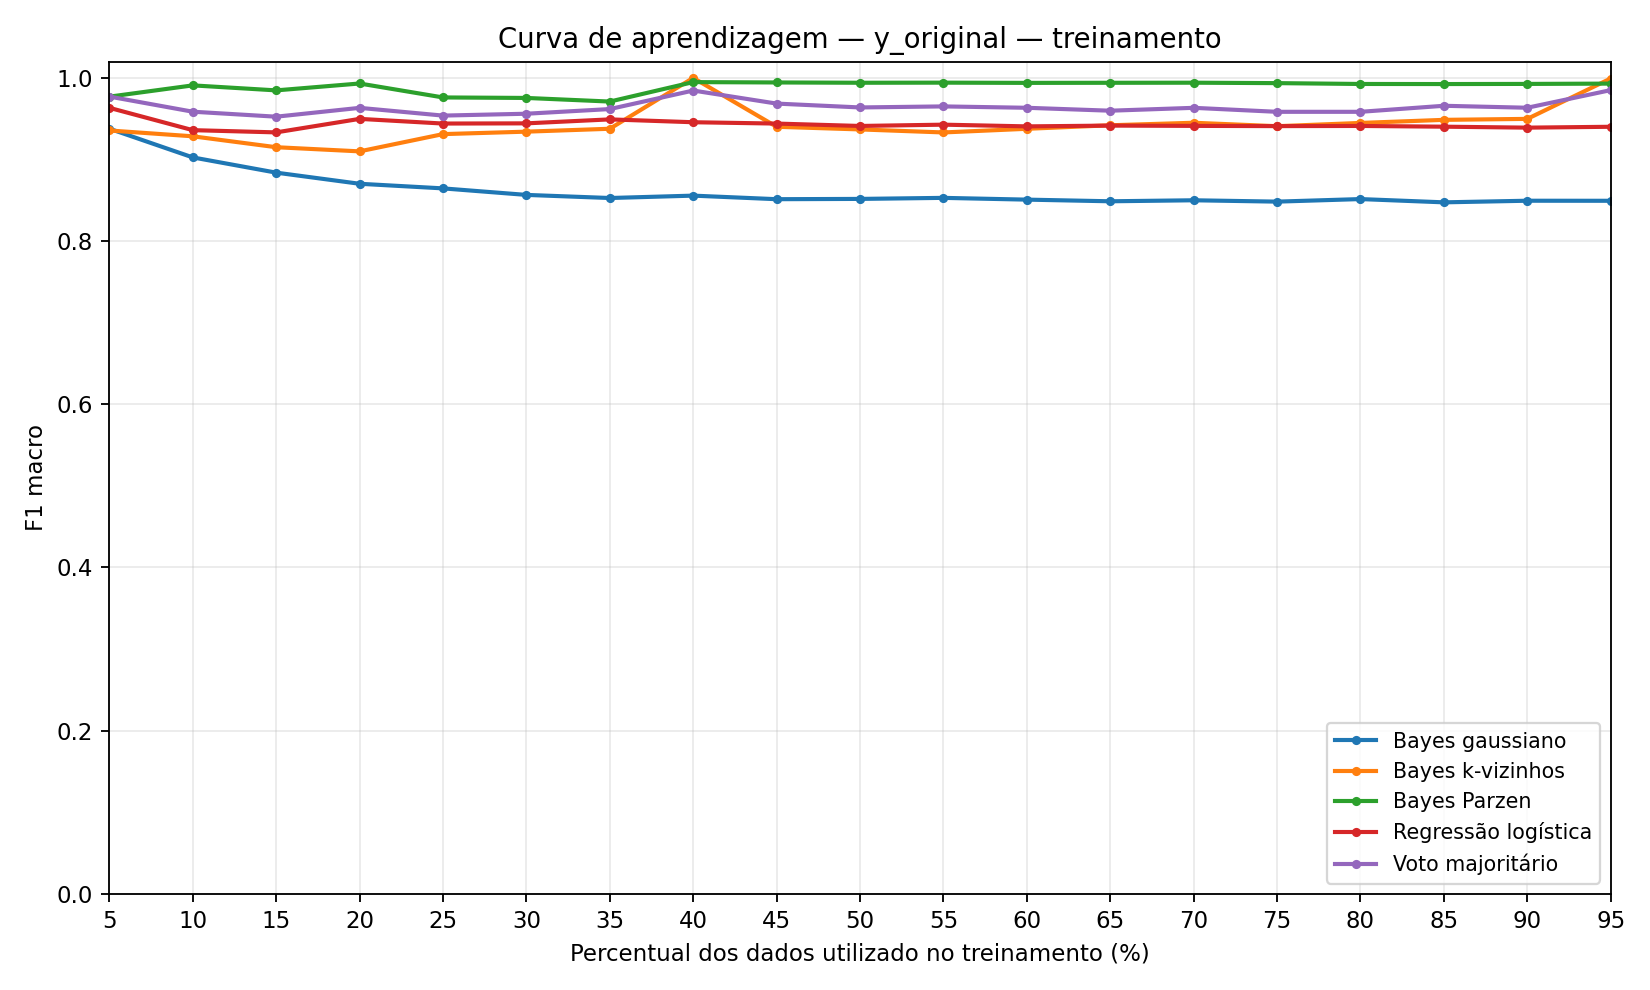
\includegraphics[width=\linewidth,height=4.45cm,keepaspectratio]{../../../questao2/resultados/curvas_aprendizagem/graficos/y_original_f1_treinamento.png}
\column{.495\textwidth}\centering\textbf{F1 de teste}\\[1mm]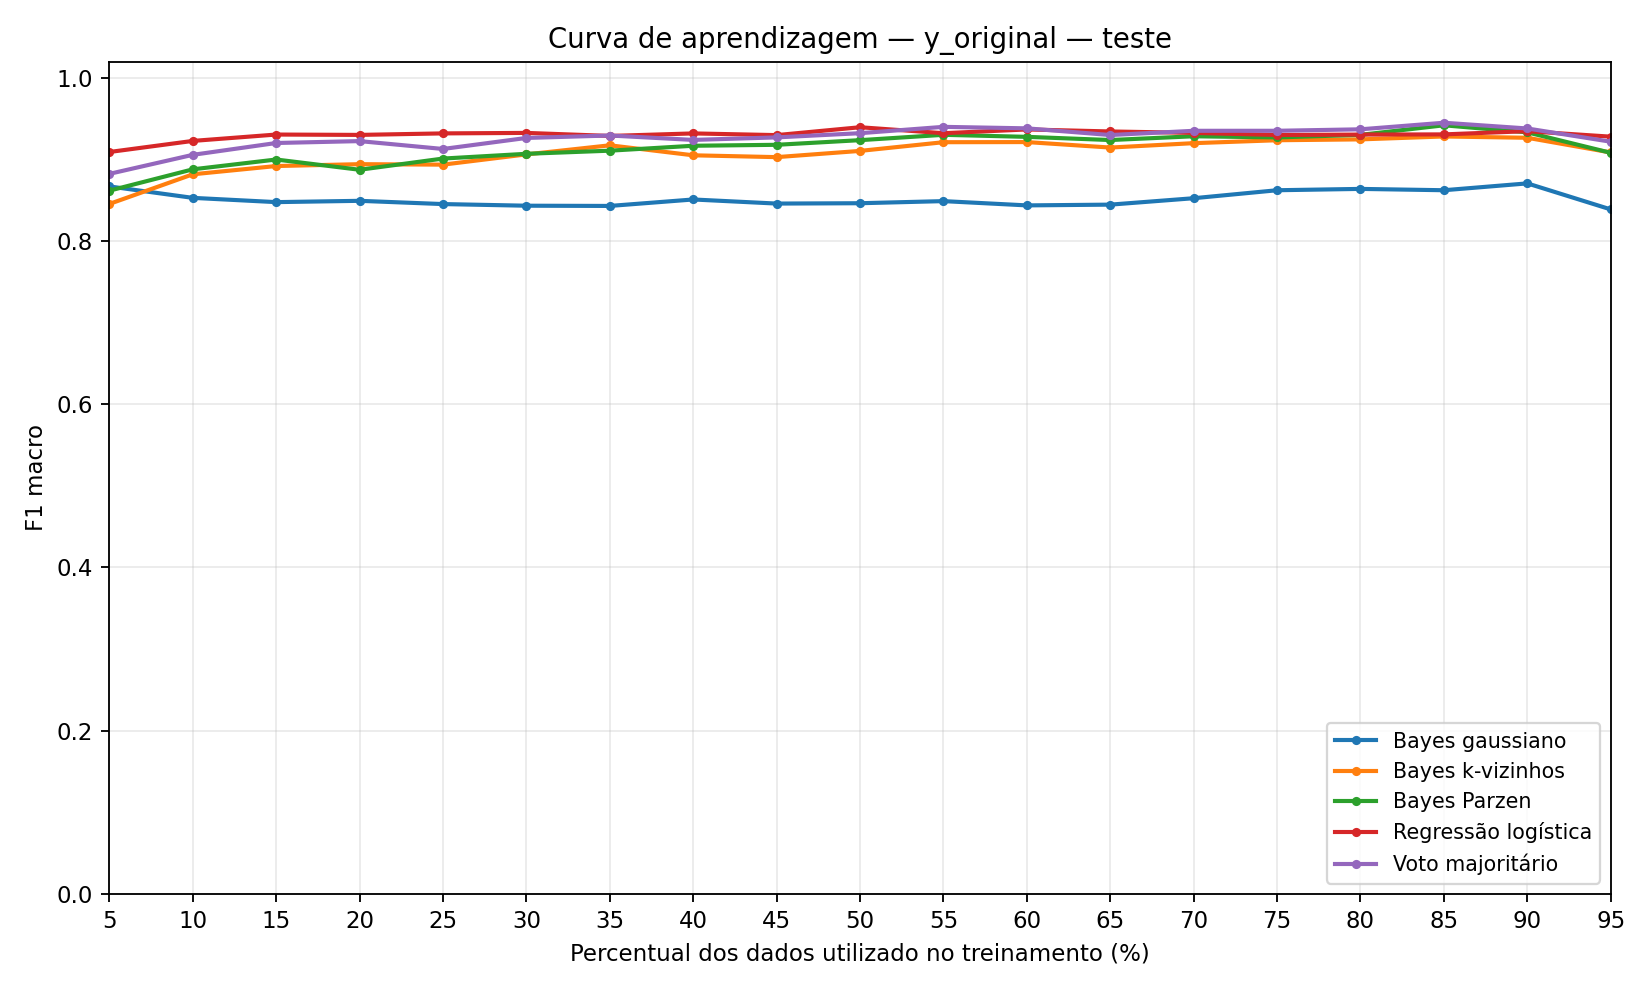
\includegraphics[width=\linewidth,height=4.45cm,keepaspectratio]{../../../questao2/resultados/curvas_aprendizagem/graficos/y_original_f1_teste.png}
\end{columns}
\vspace{1mm}
\begin{notabox}\scriptsize Parzen e k-NN têm lacuna treino--teste; Logística é competitiva já com poucas amostras. Divisões estratificadas de 5\% a 95\%, passo de 5\%; uma divisão por proporção.\end{notabox}

\end{frame}

%% PRINCIPAL 21
\begin{frame}[t]{Q2 | Curvas de aprendizagem: clusters}

\begin{columns}[T,onlytextwidth]
\column{.495\textwidth}\centering\textbf{F1 de treinamento}\\[1mm]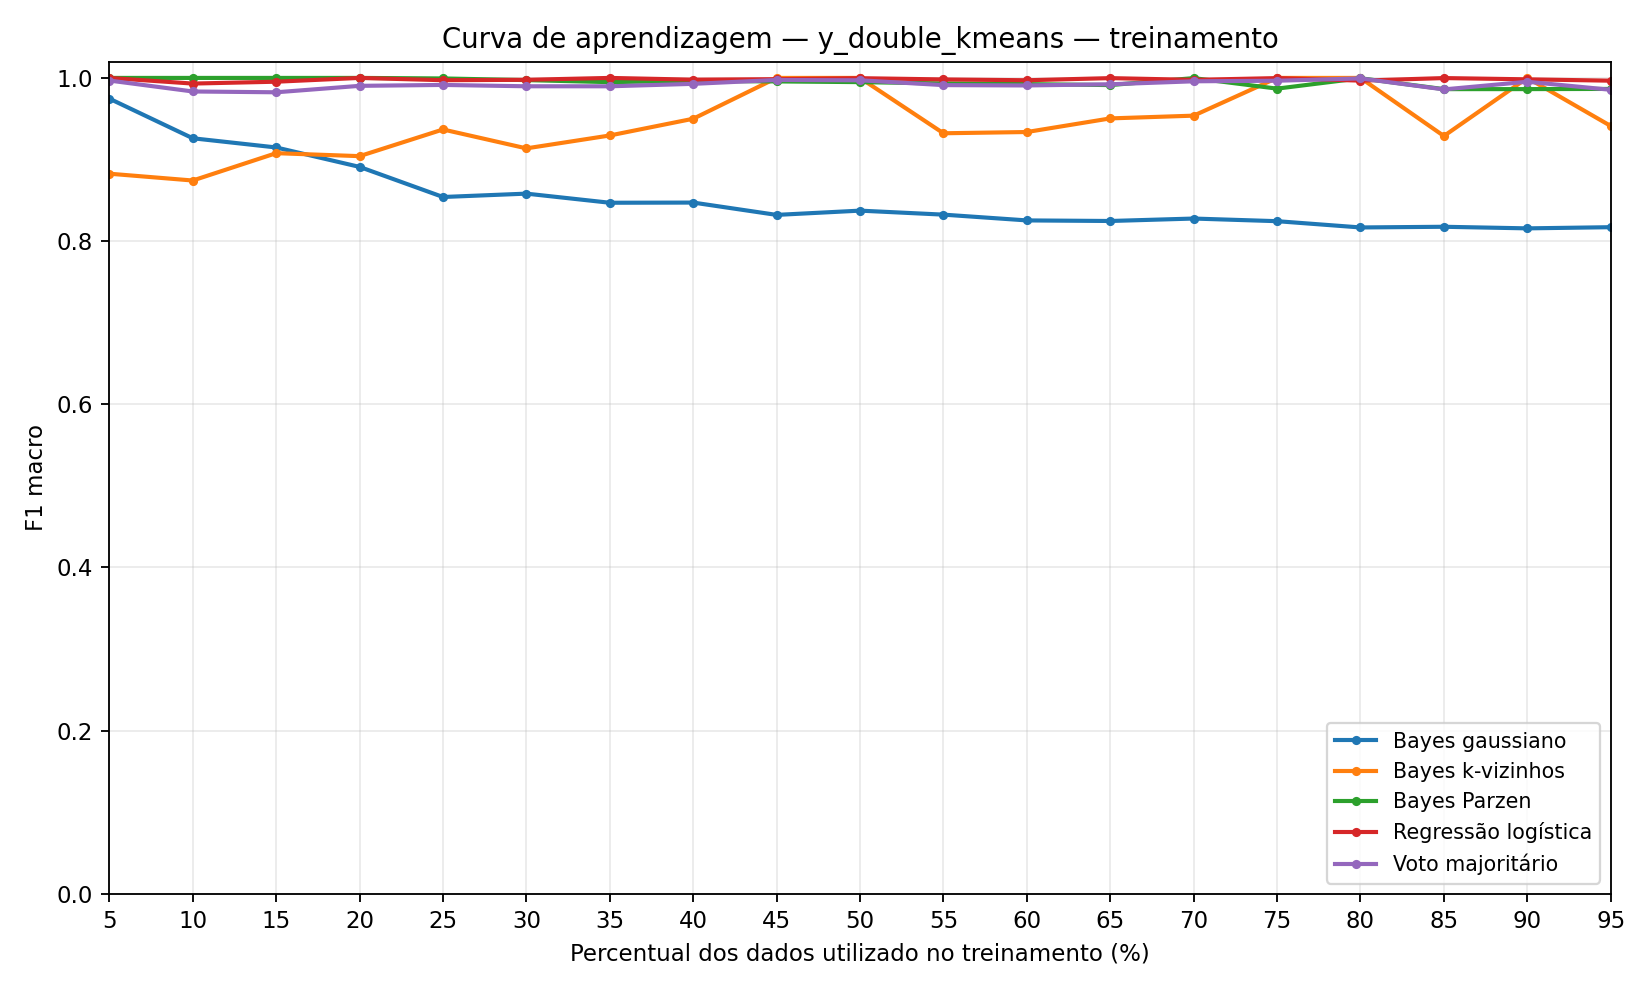
\includegraphics[width=\linewidth,height=4.45cm,keepaspectratio]{../../../questao2/resultados/curvas_aprendizagem/graficos/y_double_kmeans_f1_treinamento.png}
\column{.495\textwidth}\centering\textbf{F1 de teste}\\[1mm]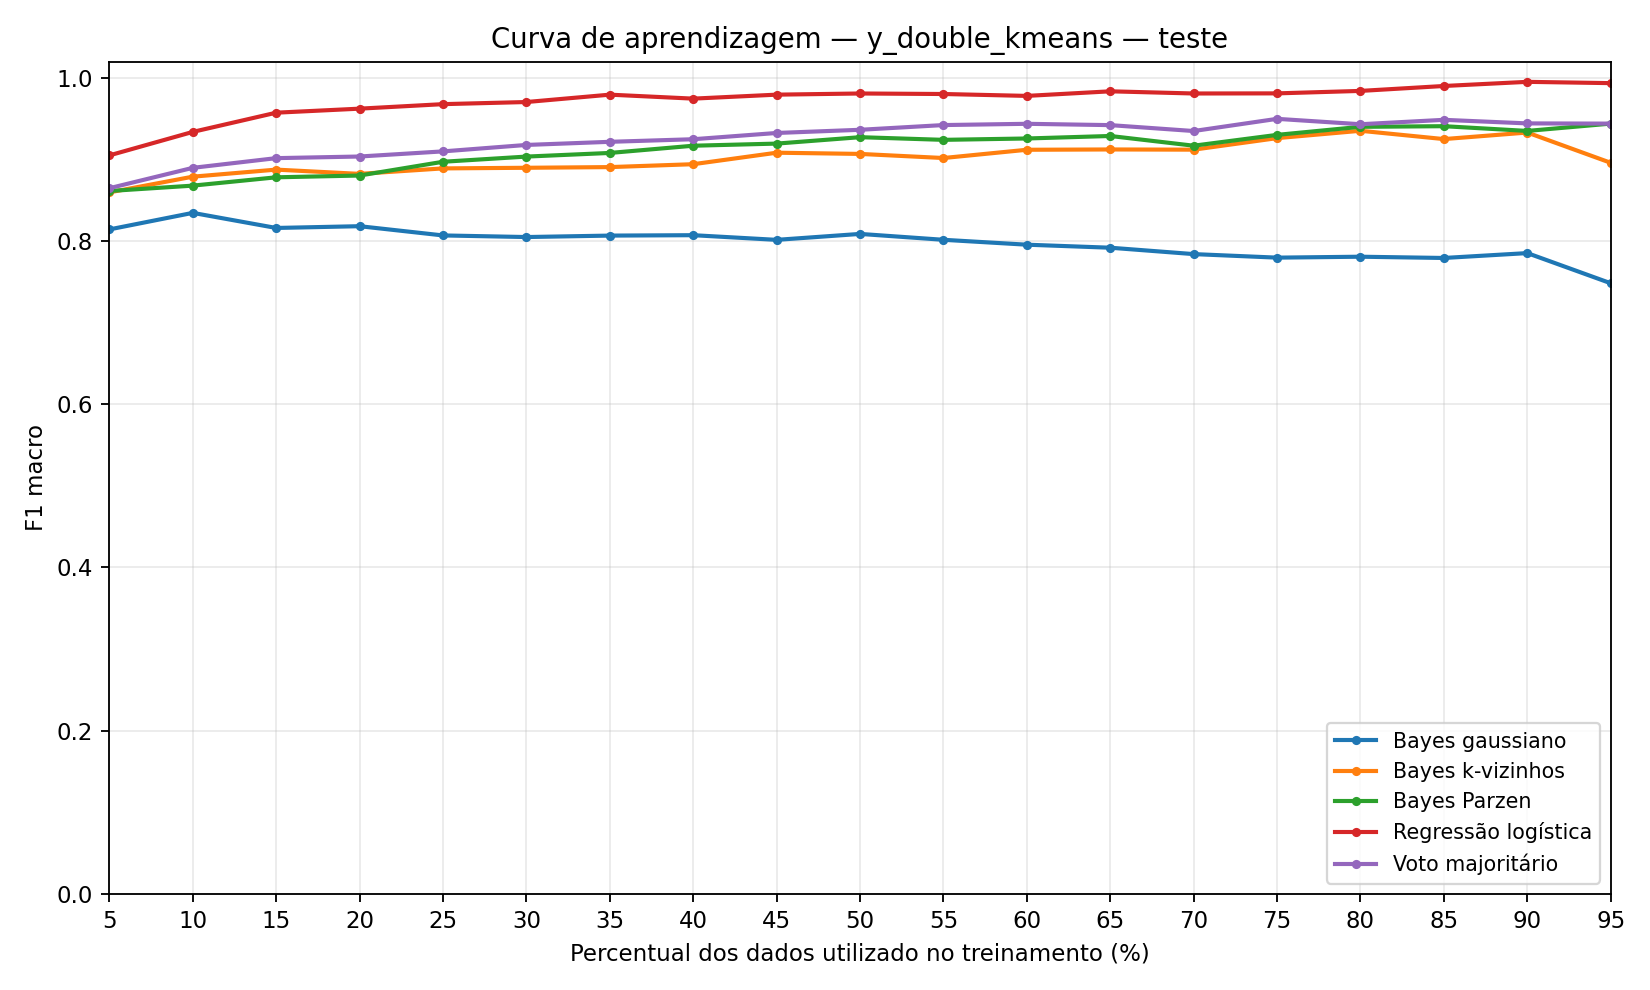
\includegraphics[width=\linewidth,height=4.45cm,keepaspectratio]{../../../questao2/resultados/curvas_aprendizagem/graficos/y_double_kmeans_f1_teste.png}
\end{columns}
\vspace{1mm}
\begin{notabox}\scriptsize A Logística atinge F1 de teste $0,9050$ em 5\% de treino e $0,9936$ em 95\%. Divisões estratificadas de 5\% a 95\%, passo de 5\%; uma divisão por proporção.\end{notabox}

\end{frame}

%% PRINCIPAL 22
\begin{frame}[t]{Resultados e limites de interpretação}

\begin{columns}[T,onlytextwidth]
\column{.5\textwidth}\begin{simplebox}
\textbf{O que os experimentos mostram}\par\smallskip
\small \textbf{Q1:} $K^*=3$ em \texttt{log\_minmax}, ARI $0,3911$.\par\smallskip
\small \textbf{Q2 original:} Voto e Parzen lideram em F1 macro ($\approx 0,94$).\par\smallskip
\small \textbf{Q2 clusters:} Logística lidera em F1 ($0,9827$).
\end{simplebox}
\column{.47\textwidth}\begin{alertabox}
\textbf{Limites}\par\smallskip
\scriptsize 1. Representação de Q1 escolhida também com ARI: não totalmente cega aos rótulos.\par\smallskip
2. Alvos de 2 e 3 classes são tarefas diferentes.\par\smallskip
3. ICs e testes são \textbf{exploratórios}: os 30 blocos reutilizam as mesmas observações.\par\smallskip
4. Rótulos dos clusters foram obtidos sobre toda a base.
\end{alertabox}\end{columns}

\end{frame}

%% PRINCIPAL 23
\begin{frame}[t]{Obrigado! | Discussão}

\vspace{1.1cm}\begin{center}
{\fontsize{24}{28}\selectfont\bfseries\color{cinazul}Spambase: do Double K-means à classificação}
\vspace{6mm}\par
\small\textbf{Resultados verificáveis, protocolo reproduzível e conclusões com ressalvas.}
\vspace{7mm}\par
\scriptsize Slides seguintes: apêndice técnico para consulta durante as perguntas.
\end{center}

\end{frame}

\appendix

%% APOIO 24
\begin{frame}[t]{Apoio A | Grade completa de $(K,H)$: log1p + MinMax}

\small A escolha é a Silhueta máxima \textbf{depois} da seleção do menor $W$ nos 100 reinícios de cada par.\vspace{2mm}
\par
\scriptsize
\renewcommand{\arraystretch}{1.03}
\setlength{\tabcolsep}{4pt}
\centering
\begin{tabular}{ccc}
\toprule
Par $(K,H)$ & Silhueta & Função objetivo $W$ \\
\midrule
$(2,1)$ & 0,12588 & 4300,96 \\
$(2,2)$ & 0,10900 & 3127,15 \\
$(3,1)$ & 0,04962 & 4268,59 \\
$(3,2)$ & 0,06440 & 3091,83 \\
$(3,3)$ & 0,12922 & 2906,23 \\
$(4,1)$ & 0,02426 & 4256,96 \\
$(4,2)$ & 0,06633 & 3043,45 \\
$(4,3)$ & 0,06790 & 2829,13 \\
$(4,4)$ & 0,07141 & 2715,64 \\
\bottomrule
\end{tabular}
\par
\vspace{2mm}\begin{notabox}\scriptsize $(3,3)$ vence por Silhueta $0,129219$ e corresponde a $W=2.906,230738$.\end{notabox}

\end{frame}

%% APOIO 25
\begin{frame}[t]{Apoio B | Linha de base e microcluster espúrio}

\begin{columns}[T,onlytextwidth]
\column{.49\textwidth}\centering\textbf{Silhueta, z-score puro}\\[2mm]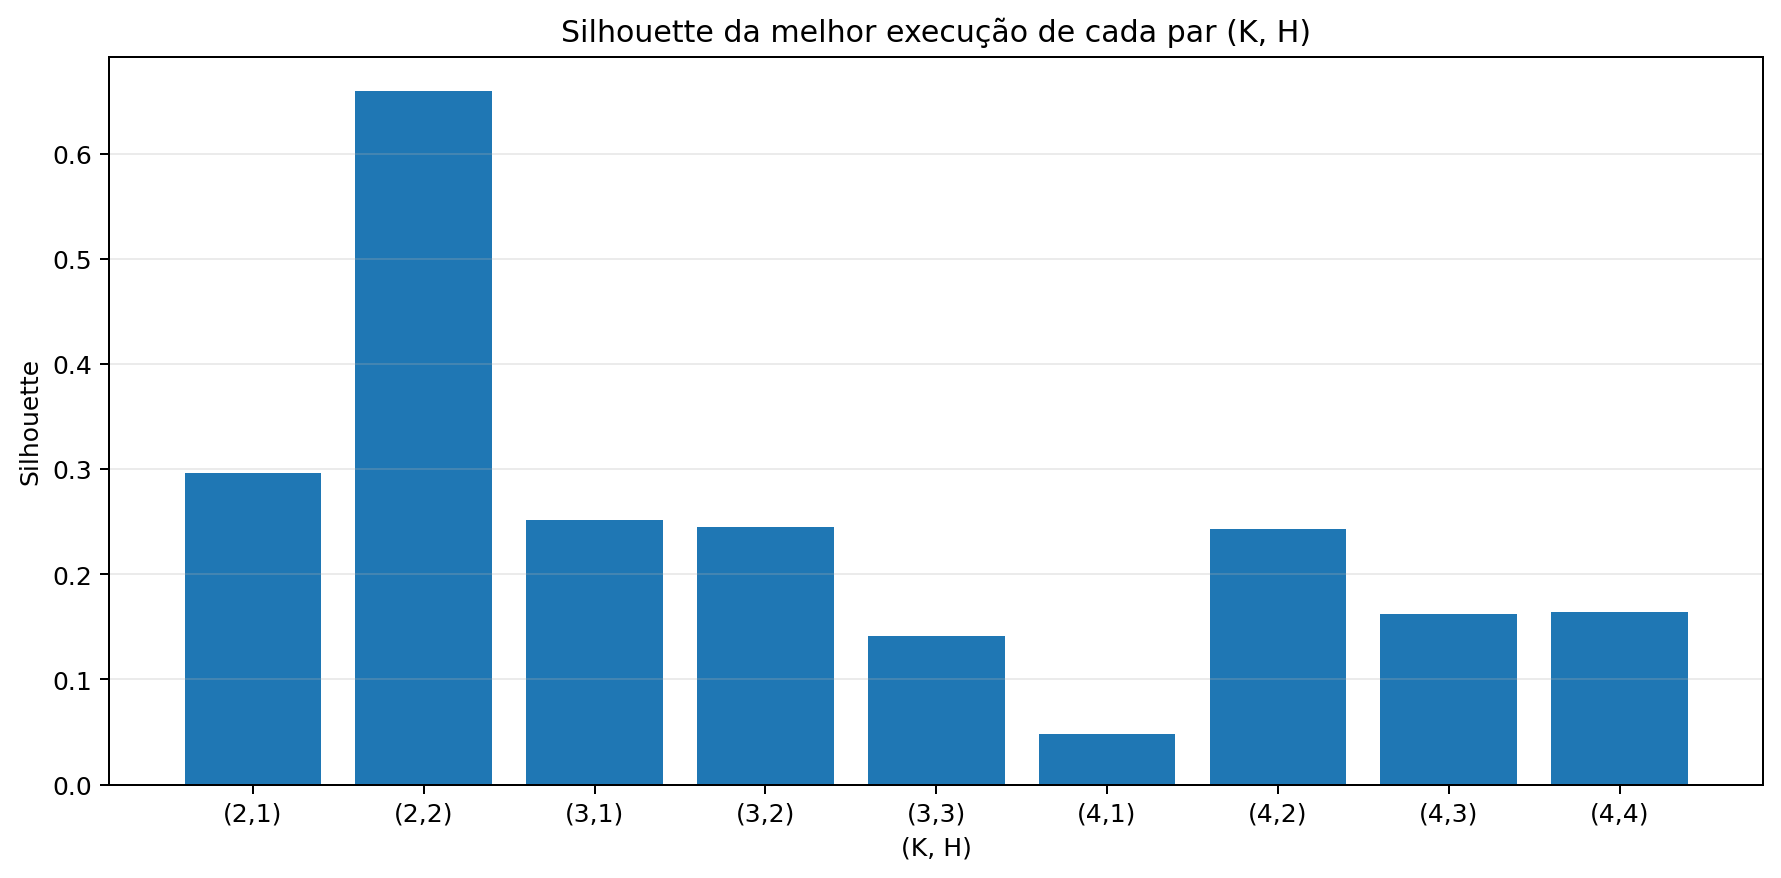
\includegraphics[width=\linewidth,height=4.5cm,keepaspectratio]{../../../questao1/resultados/revisada/silhouette_KH.png}
\column{.49\textwidth}\centering\textbf{Contingência, z-score puro}\\[2mm]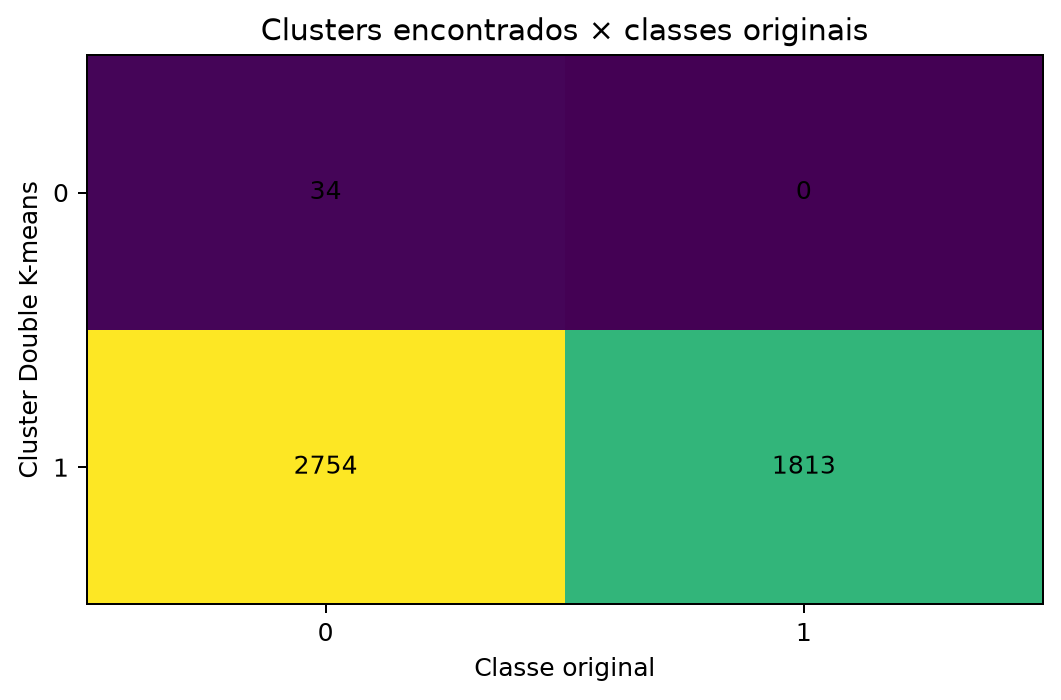
\includegraphics[width=\linewidth,height=4.5cm,keepaspectratio]{../../../questao1/resultados/originais/matriz_contingencia.png}
\end{columns}
\vspace{1mm}\scriptsize $(K^*,H^*)=(2,2)$; Silhueta $0,659631$, ARI $-0,004950$; 34 não-spams isolados e 4.567 demais.

\end{frame}

%% APOIO 26
\begin{frame}[t]{Apoio C | Os protótipos da linha de base}

\small $G$ estimado nos atributos z-score, com a partição vencedora $(2,2)$.\vspace{3mm}
\par
\small
\renewcommand{\arraystretch}{1.6}
\setlength{\tabcolsep}{4pt}
\centering
\begin{tabular}{lcc}
\toprule
Grupo de objetos & 11 termos técnicos & 46 outras variáveis \\
\midrule
Cluster 0: 34 e-mails & \textbf{+6,861185} & -0,144405 \\
Cluster 1: 4.567 e-mails & -0,051080 & +0,001075 \\
\bottomrule
\end{tabular}
\par
\vspace{3mm}
\begin{notabox}\small \textbf{Contingência:} Cluster 0 = 34 não-spam / 0 spam; Cluster 1 = 2.754 não-spam / 1.813 spam.\end{notabox}
\vspace{2mm}\begin{alertabox}\small A distância extrema em poucos termos do domínio (HP Labs) elevou a Silhueta, mas a divisão não recuperou a estrutura spam/não-spam.\end{alertabox}

\end{frame}

%% APOIO IC
\begin{frame}[t]{Apoio D | ICs de 95\%: classes originais}

\scriptsize Cada célula: média e IC95\% descritivo por t de Student (30 médias de repetição).\vspace{2mm}
\par
\scriptsize
\renewcommand{\arraystretch}{1.35}
\setlength{\tabcolsep}{4pt}
\centering
\begin{tabular}{lcccc}
\toprule
Modelo & Erro $\downarrow$ & Precisão $\uparrow$ & Cobertura $\uparrow$ & F1 $\uparrow$ \\
\midrule
Gaussiano & \shortstack{15,16\%\\{\tiny [15,11; 15,21]\%}} & \shortstack{0,8525\\{\tiny [0,8520; 0,8529]}} & \shortstack{0,8683\\{\tiny [0,8678; 0,8688]}} & \shortstack{0,8471\\{\tiny [0,8466; 0,8476]}} \\
Bayes k-NN & \shortstack{6,74\%\\{\tiny [6,67; 6,82]\%}} & \shortstack{0,9321\\{\tiny [0,9313; 0,9329]}} & \shortstack{0,9266\\{\tiny [0,9257; 0,9274]}} & \shortstack{0,9290\\{\tiny [0,9282; 0,9298]}} \\
Bayes Parzen & \shortstack{5,75\%\\{\tiny [5,70; 5,81]\%}} & \shortstack{0,9422\\{\tiny [0,9416; 0,9428]}} & \shortstack{0,9372\\{\tiny [0,9366; 0,9378]}} & \shortstack{0,9394\\{\tiny [0,9389; 0,9400]}} \\
Logística & \shortstack{6,16\%\\{\tiny [6,12; 6,20]\%}} & \shortstack{0,9357\\{\tiny [0,9352; 0,9361]}} & \shortstack{0,9359\\{\tiny [0,9354; 0,9364]}} & \shortstack{0,9355\\{\tiny [0,9351; 0,9360]}} \\
Voto & \shortstack{5,71\%\\{\tiny [5,66; 5,76]\%}} & \shortstack{0,9439\\{\tiny [0,9434; 0,9444]}} & \shortstack{0,9364\\{\tiny [0,9358; 0,9370]}} & \shortstack{0,9397\\{\tiny [0,9392; 0,9402]}} \\
\bottomrule
\end{tabular}
\par
\vspace{3mm}\begin{notabox}\scriptsize Não interpretar como IC inferencial estrito para novas amostras independentes: as 30 repetições compartilham as mesmas observações.\end{notabox}

\end{frame}

%% APOIO IC
\begin{frame}[t]{Apoio E | ICs de 95\%: clusters}

\scriptsize Cada célula: média e IC95\% descritivo por t de Student (30 médias de repetição).\vspace{2mm}
\par
\scriptsize
\renewcommand{\arraystretch}{1.35}
\setlength{\tabcolsep}{4pt}
\centering
\begin{tabular}{lcccc}
\toprule
Modelo & Erro $\downarrow$ & Precisão $\uparrow$ & Cobertura $\uparrow$ & F1 $\uparrow$ \\
\midrule
Gaussiano & \shortstack{16,99\%\\{\tiny [16,93; 17,04]\%}} & \shortstack{0,7624\\{\tiny [0,7616; 0,7632]}} & \shortstack{0,8774\\{\tiny [0,8768; 0,8781]}} & \shortstack{0,7976\\{\tiny [0,7968; 0,7984]}} \\
Bayes k-NN & \shortstack{6,55\%\\{\tiny [6,46; 6,63]\%}} & \shortstack{0,9392\\{\tiny [0,9376; 0,9408]}} & \shortstack{0,8903\\{\tiny [0,8883; 0,8922]}} & \shortstack{0,9114\\{\tiny [0,9099; 0,9129]}} \\
Bayes Parzen & \shortstack{5,66\%\\{\tiny [5,61; 5,71]\%}} & \shortstack{0,9521\\{\tiny [0,9510; 0,9532]}} & \shortstack{0,9000\\{\tiny [0,8990; 0,9011]}} & \shortstack{0,9224\\{\tiny [0,9217; 0,9232]}} \\
Logística & \shortstack{0,95\%\\{\tiny [0,92; 0,98]\%}} & \shortstack{0,9840\\{\tiny [0,9832; 0,9848]}} & \shortstack{0,9819\\{\tiny [0,9810; 0,9828]}} & \shortstack{0,9827\\{\tiny [0,9821; 0,9833]}} \\
Voto & \shortstack{4,64\%\\{\tiny [4,59; 4,69]\%}} & \shortstack{0,9612\\{\tiny [0,9600; 0,9625]}} & \shortstack{0,9141\\{\tiny [0,9129; 0,9153]}} & \shortstack{0,9347\\{\tiny [0,9338; 0,9357]}} \\
\bottomrule
\end{tabular}
\par
\vspace{3mm}\begin{notabox}\scriptsize Não interpretar como IC inferencial estrito para novas amostras independentes: as 30 repetições compartilham as mesmas observações.\end{notabox}

\end{frame}

%% APOIO RANKS
\begin{frame}[t]{Apoio F | Ranks de Nemenyi: classes originais}

\small Rank $1$ = melhor; $5$ = pior. Distância crítica (Nemenyi): $\mathrm{CD}=1,1136$ (5\%).\vspace{3mm}
\par
\scriptsize
\renewcommand{\arraystretch}{1.65}
\setlength{\tabcolsep}{4pt}
\centering
\begin{tabular}{lccccc}
\toprule
Métrica & Gaussiano & Bayes k-NN & Bayes Parzen & Logística & Voto \\
\midrule
Erro & 5,00 & 4,00 & 1,62 & 3,00 & 1,38 \\
Precisão & 5,00 & 3,97 & 1,83 & 3,03 & 1,17 \\
Cobertura & 5,00 & 4,00 & 1,73 & 2,33 & 1,93 \\
F1 macro & 5,00 & 4,00 & 1,60 & 3,00 & 1,40 \\
\bottomrule
\end{tabular}
\par
\vspace{3mm}\begin{notabox}\small Para declarar um par diferente pelo critério CD, a diferença absoluta dos seus ranks médios deve ser \textbf{maior que 1,1136}.\end{notabox}

\end{frame}

%% APOIO RANKS
\begin{frame}[t]{Apoio G | Ranks de Nemenyi: clusters}

\small Rank $1$ = melhor; $5$ = pior. Distância crítica (Nemenyi): $\mathrm{CD}=1,1136$ (5\%).\vspace{3mm}
\par
\scriptsize
\renewcommand{\arraystretch}{1.65}
\setlength{\tabcolsep}{4pt}
\centering
\begin{tabular}{lccccc}
\toprule
Métrica & Gaussiano & Bayes k-NN & Bayes Parzen & Logística & Voto \\
\midrule
Erro & 5,00 & 4,00 & 3,00 & 1,00 & 2,00 \\
Precisão & 5,00 & 4,00 & 3,00 & 1,00 & 2,00 \\
Cobertura & 5,00 & 3,97 & 3,03 & 1,00 & 2,00 \\
F1 macro & 5,00 & 4,00 & 3,00 & 1,00 & 2,00 \\
\bottomrule
\end{tabular}
\par
\vspace{3mm}\begin{notabox}\small Para declarar um par diferente pelo critério CD, a diferença absoluta dos seus ranks médios deve ser \textbf{maior que 1,1136}.\end{notabox}

\end{frame}

%% APOIO NEMENYI
\begin{frame}[t]{Apoio H | Nemenyi: Voto x Parzen (todas as métricas)}

\small Comparação dos dois líderes de F1 macro na tarefa correspondente.\vspace{3mm}
\par
\small
\renewcommand{\arraystretch}{1.6}
\setlength{\tabcolsep}{4pt}
\centering
\begin{tabular}{lccc}
\toprule
Métrica & $|\Delta \mathrm{rank}|$ & $p$ (Nemenyi) & Diferença detectada? \\
\midrule
Erro & 0,23 & 0,9792 & Não \\
Precisão & 0,67 & 0,4761 & Não \\
Cobertura & 0,20 & 0,9883 & Não \\
F1 macro & 0,20 & 0,9883 & Não \\
\bottomrule
\end{tabular}
\par
\vspace{3mm}\begin{notabox}\small Ausência de diferença detectada pelo pós-teste \textbf{não prova equivalência} estatística ou prática.\end{notabox}

\end{frame}

%% APOIO NEMENYI
\begin{frame}[t]{Apoio I | Nemenyi: Logística x Voto (todas as métricas)}

\small Comparação dos dois líderes de F1 macro na tarefa correspondente.\vspace{3mm}
\par
\small
\renewcommand{\arraystretch}{1.6}
\setlength{\tabcolsep}{4pt}
\centering
\begin{tabular}{lccc}
\toprule
Métrica & $|\Delta \mathrm{rank}|$ & $p$ (Nemenyi) & Diferença detectada? \\
\midrule
Erro & 1,00 & 0,1024 & Não \\
Precisão & 1,00 & 0,1024 & Não \\
Cobertura & 1,00 & 0,1024 & Não \\
F1 macro & 1,00 & 0,1024 & Não \\
\bottomrule
\end{tabular}
\par
\vspace{3mm}\begin{notabox}\small Ausência de diferença detectada pelo pós-teste \textbf{não prova equivalência} estatística ou prática.\end{notabox}

\end{frame}

%% APOIO CURVAS
\begin{frame}[t]{Apoio J | Treino x teste: classes originais}

\begin{columns}[T,onlytextwidth]
\column{.49\textwidth}\centering\textbf{Regressão Logística}\\[1mm]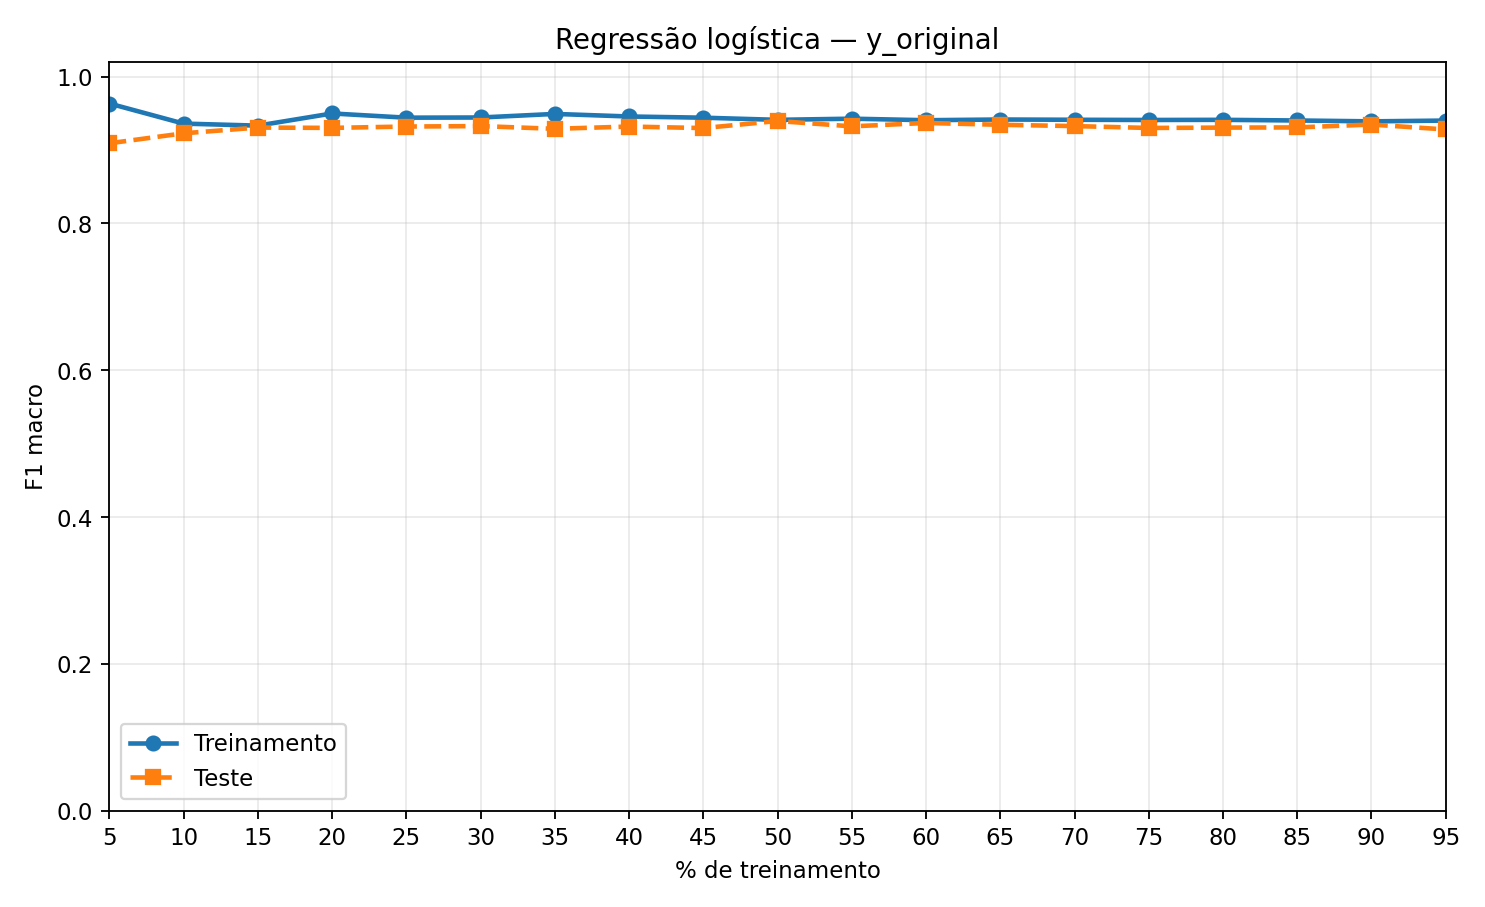
\includegraphics[width=\linewidth,height=4.65cm,keepaspectratio]{../../../questao2/resultados/curvas_aprendizagem/graficos/y_original_logistica_treino_vs_teste.png}
\column{.49\textwidth}\centering\textbf{Bayes Parzen}\\[1mm]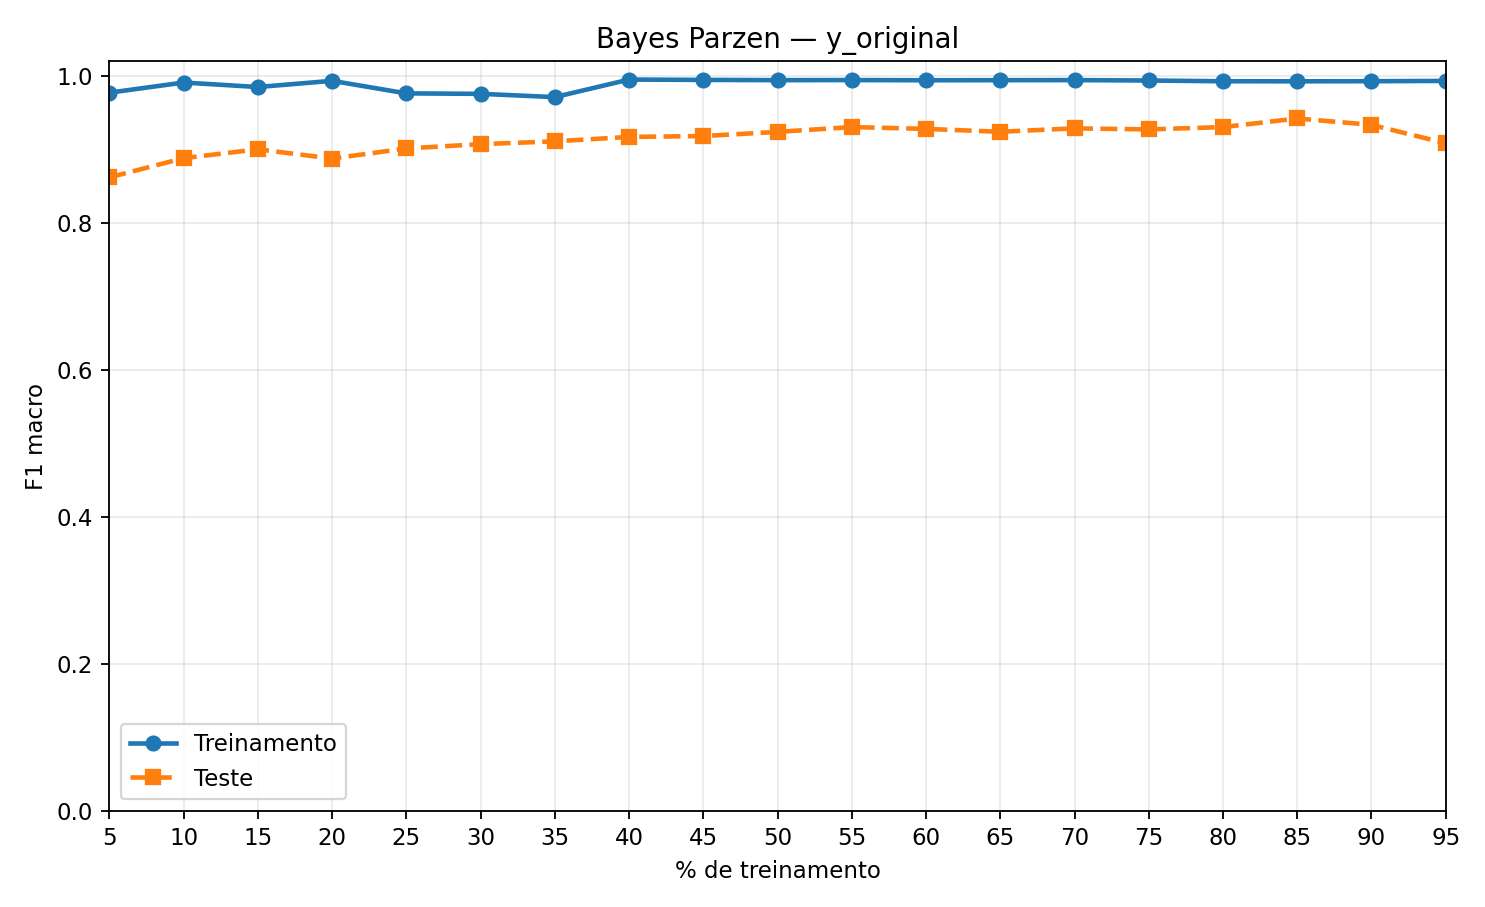
\includegraphics[width=\linewidth,height=4.65cm,keepaspectratio]{../../../questao2/resultados/curvas_aprendizagem/graficos/y_original_parzen_treino_vs_teste.png}
\end{columns}
\vspace{1mm}\begin{notabox}\scriptsize Curvas com amostra estratificada por proporção (5--95\%); uma divisão por ponto, com F1 macro de treino e teste.\end{notabox}

\end{frame}

%% APOIO CURVAS
\begin{frame}[t]{Apoio K | Treino x teste: clusters}

\begin{columns}[T,onlytextwidth]
\column{.49\textwidth}\centering\textbf{Regressão Logística}\\[1mm]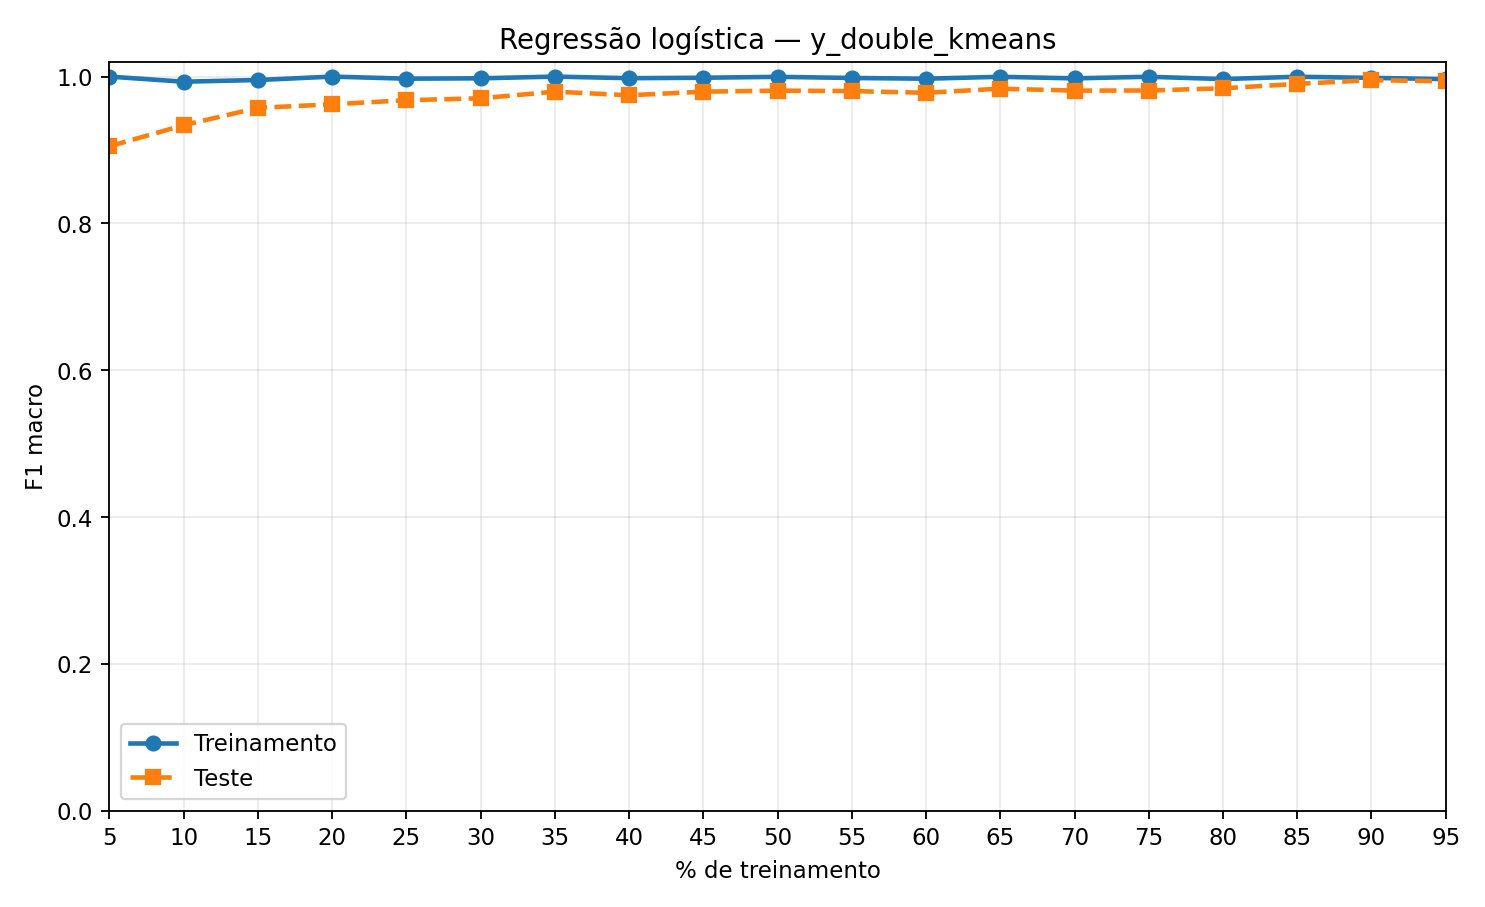
\includegraphics[width=\linewidth,height=4.65cm,keepaspectratio]{../../../questao2/resultados/curvas_aprendizagem/graficos/y_double_kmeans_logistica_treino_vs_teste.png}
\column{.49\textwidth}\centering\textbf{Bayes Parzen}\\[1mm]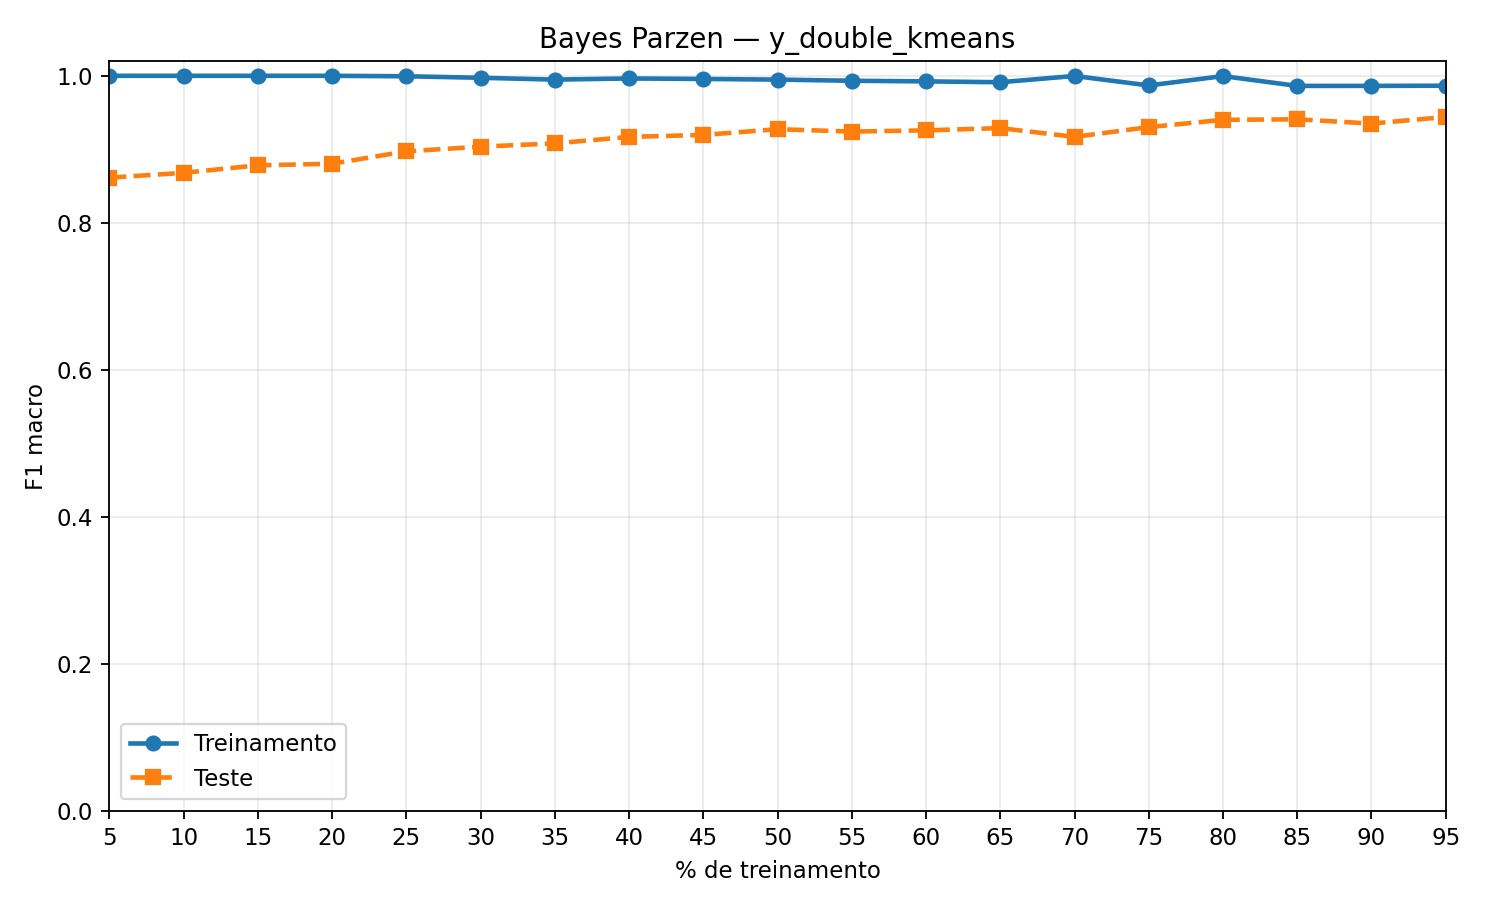
\includegraphics[width=\linewidth,height=4.65cm,keepaspectratio]{../../../questao2/resultados/curvas_aprendizagem/graficos/y_double_kmeans_parzen_treino_vs_teste.png}
\end{columns}
\vspace{1mm}\begin{notabox}\scriptsize Curvas com amostra estratificada por proporção (5--95\%); uma divisão por ponto, com F1 macro de treino e teste.\end{notabox}

\end{frame}

%% APOIO 34
\begin{frame}[t]{Apoio L | Reprodutibilidade e entregáveis}

\begin{columns}[T,onlytextwidth]
\column{.52\textwidth}
\begin{simplebox}\small\textbf{Artefatos disponíveis}\par\smallskip
\scriptsize \texttt{questao1/}: implementação, grade, 7 representações, matrizes e figuras.\par\smallskip
\scriptsize \texttt{questao2/}: 5 classificadores, CV aninhada, CSVs por fold, estatística e curvas.\par\smallskip
\scriptsize \texttt{entrega/}: relatório consolidado PDF/TeX/MD.
\end{simplebox}
\column{.45\textwidth}
\begin{simplebox}\small\textbf{Auditoria}\par\smallskip
\scriptsize $71$ testes automatizados aprovados; $43$ subtestes.\par\smallskip
\scriptsize Folds externos pareados e estratificados, sementes determinísticas, hashes de dados e registros individuais por modelo.
\end{simplebox}\end{columns}
\vspace{2mm}\begin{alertabox}\scriptsize Em 18/11/2026, a orientação do enunciado é entregar arquivos \textbf{individualmente}, sem ZIP, no Google Classroom.\end{alertabox}

\end{frame}

\begin{frame}[t]{Apoio M | Nemenyi completo: classes originais}
\scriptsize Dez pares, quatro métricas; pós-teste exploratório sobre 30 ranks médios pareados.\par\vspace{2mm}
\begin{center}
\scriptsize
\renewcommand{\arraystretch}{1.13}
\setlength{\tabcolsep}{5pt}
\begin{tabular}{lcccc}
\toprule
Par & Erro & Precisão & Cobertura & F1 macro \\
\midrule
Gaussiano / k-NN & 0,1024 & 0,0838 & 0,1024 & 0,1024 \\
Gaussiano / Parzen & $<10^{-4}$ & $<10^{-4}$ & $<10^{-4}$ & $<10^{-4}$ \\
Gaussiano / Logística & $<10^{-4}$ & $<10^{-4}$ & $<10^{-4}$ & $<10^{-4}$ \\
Gaussiano / Voto & $<10^{-4}$ & $<10^{-4}$ & $<10^{-4}$ & $<10^{-4}$ \\
k-NN / Parzen & $<10^{-4}$ & $<10^{-4}$ & $<10^{-4}$ & $<10^{-4}$ \\
k-NN / Logística & 0,1024 & 0,1493 & 0,0004 & 0,1024 \\
k-NN / Voto & $<10^{-4}$ & $<10^{-4}$ & $<10^{-4}$ & $<10^{-4}$ \\
Parzen / Logística & 0,0063 & 0,0272 & 0,5823 & 0,0055 \\
Parzen / Voto & 0,9792 & 0,4761 & 0,9883 & 0,9883 \\
Logística / Voto & 0,0007 & $<10^{-4}$ & 0,8645 & 0,0008 \\
\bottomrule
\end{tabular}
\end{center}
\vspace{2mm}
\begin{notabox}\scriptsize Rejeição pelo Nemenyi se $p<0,05$ (equivalente a diferença de rank médio maior que $\mathrm{CD}=1,1136$). Ausência de diferença detectada não significa equivalência.\end{notabox}
\end{frame}
\begin{frame}[t]{Apoio N | Nemenyi completo: clusters}
\scriptsize Dez pares, quatro métricas; pós-teste exploratório sobre 30 ranks médios pareados.\par\vspace{2mm}
\begin{center}
\scriptsize
\renewcommand{\arraystretch}{1.13}
\setlength{\tabcolsep}{5pt}
\begin{tabular}{lcccc}
\toprule
Par & Erro & Precisão & Cobertura & F1 macro \\
\midrule
Gaussiano / k-NN & 0,1024 & 0,1024 & 0,0838 & 0,1024 \\
Gaussiano / Parzen & $<10^{-4}$ & $<10^{-4}$ & $<10^{-4}$ & $<10^{-4}$ \\
Gaussiano / Logística & $<10^{-4}$ & $<10^{-4}$ & $<10^{-4}$ & $<10^{-4}$ \\
Gaussiano / Voto & $<10^{-4}$ & $<10^{-4}$ & $<10^{-4}$ & $<10^{-4}$ \\
k-NN / Parzen & 0,1024 & 0,1024 & 0,1493 & 0,1024 \\
k-NN / Logística & $<10^{-4}$ & $<10^{-4}$ & $<10^{-4}$ & $<10^{-4}$ \\
k-NN / Voto & $<10^{-4}$ & $<10^{-4}$ & $<10^{-4}$ & $<10^{-4}$ \\
Parzen / Logística & $<10^{-4}$ & $<10^{-4}$ & $<10^{-4}$ & $<10^{-4}$ \\
Parzen / Voto & 0,1024 & 0,1024 & 0,0838 & 0,1024 \\
Logística / Voto & 0,1024 & 0,1024 & 0,1024 & 0,1024 \\
\bottomrule
\end{tabular}
\end{center}
\vspace{2mm}
\begin{notabox}\scriptsize Rejeição pelo Nemenyi se $p<0,05$ (equivalente a diferença de rank médio maior que $\mathrm{CD}=1,1136$). Ausência de diferença detectada não significa equivalência.\end{notabox}
\end{frame}
\end{document}
